Consider a smart city that aims at being energy self-sustainable and produce and consume as much as possible, energy within its geographic area. 
Producers are characterized according to their location, the amount of energy in kWatts-hour that they can sell, the cost, and the time window in which they can produce it, with a given service level agreement concerning their availability and fault tolerance. 
Consumers, give also their location, their energy requirements during a certain interval of time, the maximum total cost they are ready to pay, and quality of service requirements such as availability and how critical it is to consume this amount of energy. 
A energy exchange market is established in order to continuously trade  energy provision/consumption ensuring that all consumers will have the energy they require at every moment.

\begin{figure*}
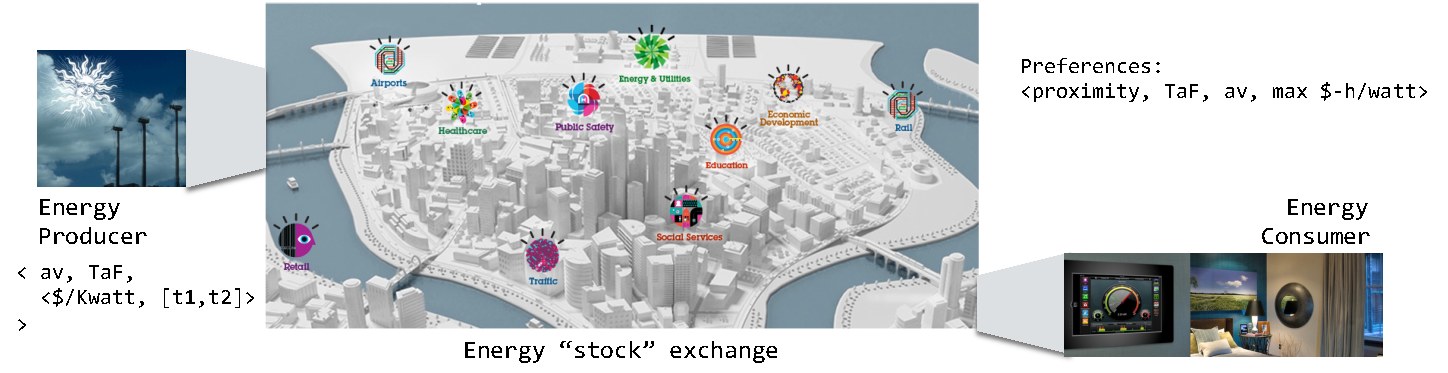
\includegraphics[width=0.95\textwidth]{figs/exchange.pdf}
\caption{\label{fig:energyXChange} Energy exchange.}
\end{figure*}

In our approach energy producers are modelled as services with associated ``agreed'' SLAs. 
In general, we assume that several producers will be able to supply energy for a given period of time given specific  preferences expressed by a consumer. 
An energy request is expressed as a query that specifies an energy requirement with QoS preferences independently of the possible producers. In our example assume that there are several energy provision services ({\sf e$_1$, ... e$_n$}) that can be independent or hubs integrating several energy providers:
\begin{description}
\sf\footnotesize
\item energyProvider.requestAvailability() $\rightarrow$ $\langle$KWatt/h, Ecost, rate, location$\rangle$

\item energyHub.requestAvailability() $\rightarrow$  \{$\langle$ID, KWatt/h, cost, rate, location$\rangle$\}

\end{description}

Each service is deployed in different cloud provider and each exports an agreed SLA that specifies the economic cost per call, the maximum number of calls that can be done per day, the disponibility of the service, the average response time when a method is called, the reliability, the privace of the produced data (whether they can be stored or not), the precision,freshness and provenance of the produced data. As said in previous sections, some of these measures ({\sf cost/call, maxCall/day}) are static and explicitly specified by the service provider. In contrast, the other measures are constantly computed by monitoring the conversations between the service and the applications that contact it.  Cloud providers define also their SLA contracts defining normally subscription contracts that specify, the cost per request ({\sf cost/request}), the volume of data that can be exchanged per month ({\sf I/0 volume/month}), the cost of transfering data or applications within the same data centre or between data centres ({\sf datatransferCost/region}), the storage space ({\sf storageSpace}). For exmaple some cloud providers enable the customer to choose the zone to install PaaS services and deploy applications (e.g. zone 1 is Europe). If the customer wishes to deploy services in zone 1 but store data in zone 2 the transfer cost will change.

\begin{description}
\sf\footnotesize
 \item {\sf agreedSLA:$\langle$cost/call, maxCalls/day, availability, responseTime, reliability, privacy, precision, freshness, provenance$\rangle$}. 
 
 \item  {\sf cloudSLA:$\langle$cost/request, I/0 volume/month, datatransferCost/region, storageSpace$\rangle$}. 
 \end{description}
 

 Given a query, expressed as an SQL like expression including spatio-temporal attributes and preferences, for example, {\em List of energy providers that can provision 1000 Kwatts/h, in the next 10 seconds, that are close to my city with a cost of 0,50 euros/Kwatt and that are labeled as green?}. The user preferences statement, includes her cloud provider contract and her quality preferences. 
 \begin{description}
\sf\footnotesize
 
 \item  {\sf cloudSLA:$\langle$0,05 cents per call, 8 Gigabytes I/0 volume/month, free, 1 Giga$\rangle$}. 
 
 \item {\sf preferencesStatement:$\langle$cost/call, maxCalls/day, availability, responseTime, reliability, privacy, precision, freshness, provenance$\rangle$}. 
 
 \end{description}
 We consider a simplified SLA cloud contract inspired in the lowest contract provided by Azure with {\sf 0,05 cents per call,  8 Gigabytes of I/O volume/month, free data transfert cost within the same region,  Gigabyte of storage}. The user is ready to pay maximum {\sf 5 euros as total query cost}, she wants only {\sf green} energy providers (provenance), at least {\sf 85$\%$} of precision of provided data, even if they are not fresh, she wants at least {\sf 90$\%$} available services, with a response time of {\sf 0,01 seconds}.
 
 Assume that there are four civilian energy providers are represented by services  {\sf e$_1$, ... e$_4$} and two {\sf hub}s which are also services integrating energy providers communities {\sf h$_1$ and h$_2$}; there are two free location services exporting  the following interface {\sf loc(IP) $\leftarrow$ $\langle$ X, Y$\rangle$} meaning that given an IP address it returns the geographic position expresses as {\sf X} and {\sf Y}. This services can potentially be combined for answering the query. 
 
 \paragraph{Derived SLA} Som of the user preferences statement measures are used for defining a dervied SLA that, as said in previous section, will guide the evaluation of the query. These measures are defined as a function of the measures used by the agreed SLAs and by the cloud SLA contract.
 
  \paragraph{Computing service compositions}
  
   \paragraph{Optimizing service compositions execution}
 